\documentclass{standalone}
\makeatletter\AtBeginDocument{\@buildstepset{1,2}}\makeatother
\usepackage{hsbcommon}
\usetikzlibrary{fit}
\begin{document}
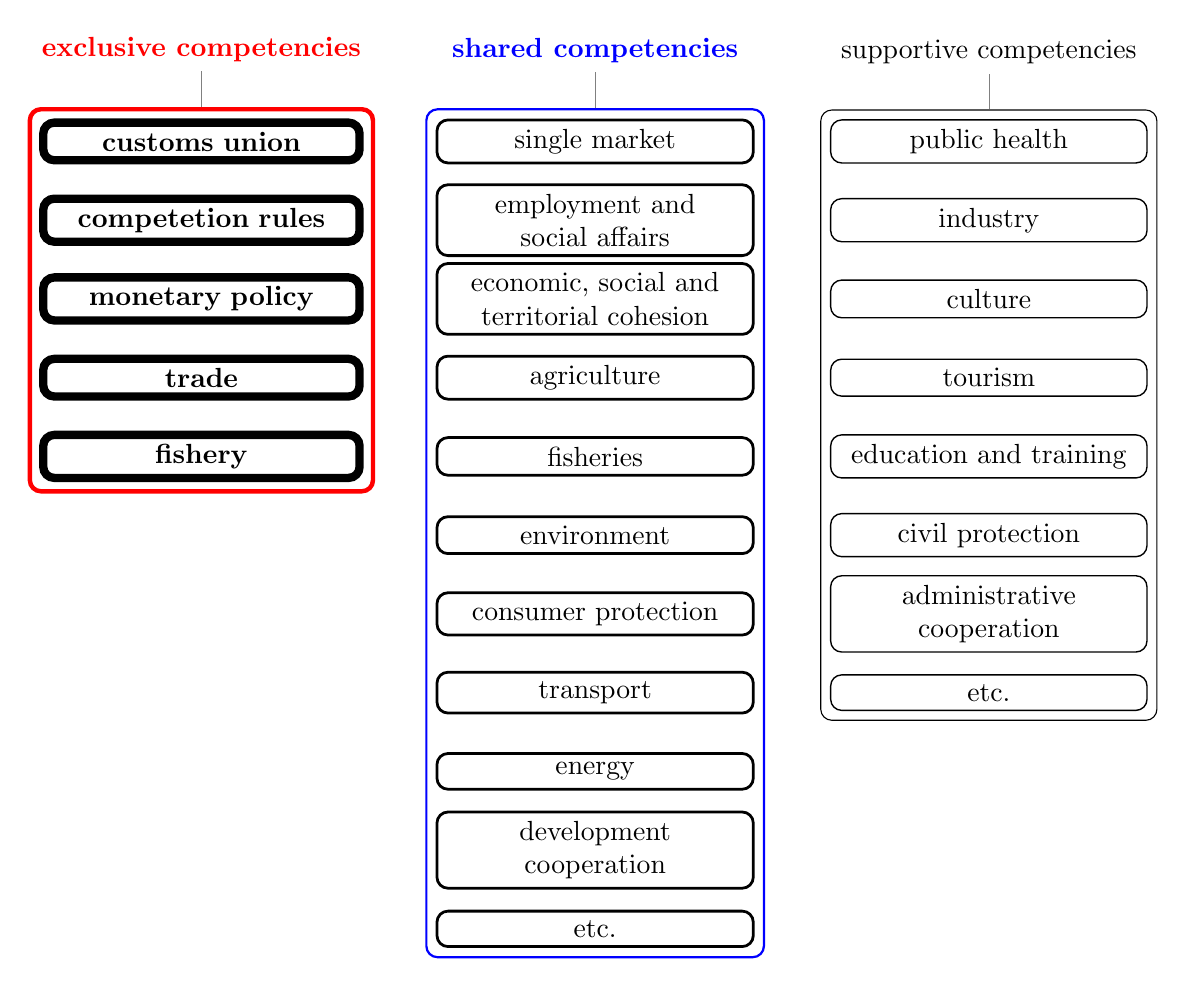
\begin{tikzpicture}
    \tikzset{
        comp/.style={
            draw,
            rounded corners,
            text width=25ex,
            align=center
        }
    }

    \ifstep{1}{ %%% exclusive competencies
        \foreach [count=\i] \myexclusive in {
            customs union,
            competetion rules,
            monetary policy,
            trade,
            fishery
        }
        {
            \node[comp,line width=3pt] (ex\i) at (0,-\i) {\textbf{\myexclusive}};
        }
        \begin{scope}[red]
            \node[draw,fit={(ex1) (ex5)},pin=\textbf{exclusive competencies},ultra thick,rounded corners] {};
        \end{scope}
        
    }

    \ifstep{2}{%%% shared competencies
    
    
        \foreach [count=\i] \myshared in {
            single market,
            employment and social affairs,
            economic{,} social and territorial cohesion,
            agriculture,
            fisheries,
            environment,
            consumer protection,
            transport,
            energy,
            development cooperation,
            etc.
        }
        {
            \node[comp,line width=1pt] (sh\i) at (5,-\i) {\myshared};
        }
    }
    \ifstep{3}{

    %%% supportive competencies

        \foreach [count=\i] \mysupportive in {
        public health,
        industry,
        culture,
        tourism,
        education and training,
        civil protection,
        administrative cooperation,
        etc.
    }
    {
        \node[comp,line width=0.5pt] (sup\i) at (10,-\i) {\mysupportive};
    }

    \begin{scope}[blue]
        \node[draw,fit={(sh1) (sh11)},pin=\textbf{shared competencies},thick,rounded corners] {};
    \end{scope}
    
    \begin{scope}[black]
        \node[draw,fit={(sup1) (sup8)},pin={supportive competencies},rounded corners] {};
    \end{scope}
    }
    
\end{tikzpicture}
\end{document}

\begin{frame}{European Union - Exclusive Competencies}
    \mytext{    
    Art. 2 TFEU: competencies

    \textbf{Exclusive competencies} (complete list):
    \begin{enumerate}
        \item \textbf{customs union}
        \item \textbf{competetion rules} for the single market
        \item \textbf{monetary policy} for the eurozone countries
        \item \textbf{trade} and international agreement (under certain circumstances)
        \item marine plants and animals regulated by the common fishery policy
    \end{enumerate}    
    }
\end{frame}

\begin{frame}{European Union - Shared Competencies}
    \mytext{
    \textbf{Shared competencies} (among others):
    \begin{itemize}
        \item single market
        \item employment and social affairs
        \item economic, social and territorial cohesion
        \item agriculture
        \item fisheries
        \item environment
        \item consumer protection
        \item transport
        \item energy
        \item development cooperation
        \item ...
    \end{itemize}    
    }
\end{frame}

\begin{frame}{European Union - Supporting Competencies}
    \mytext{
    \textbf{Supporting competencies:}
    \begin{itemize}
        \item public health
        \item industry
        \item culture
        \item tourism
        \item education and training
        \item civil protection
        \item administrative cooperation
        \item ...
    \end{itemize}

    \bigskip

    Also: \textit{special} competencies (EU's common foreign and secutiry policy, etc.)    
    }
\end{frame}